\textbf{~{1. 两个有序链表合并为一个有序链表}}

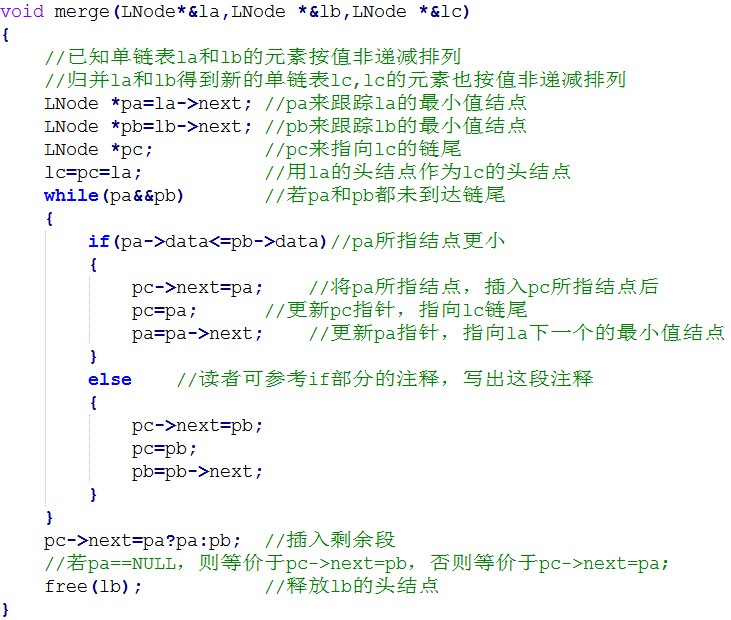
\includegraphics[width=3.12500in,height=2.64583in]{png-jpeg-pics/27B36B8E0380485A33092BEA1B313D5E.png}

\textbf{{2. 查找链表L中值为key的结点,存在就删除并返回1,否则返回0}}

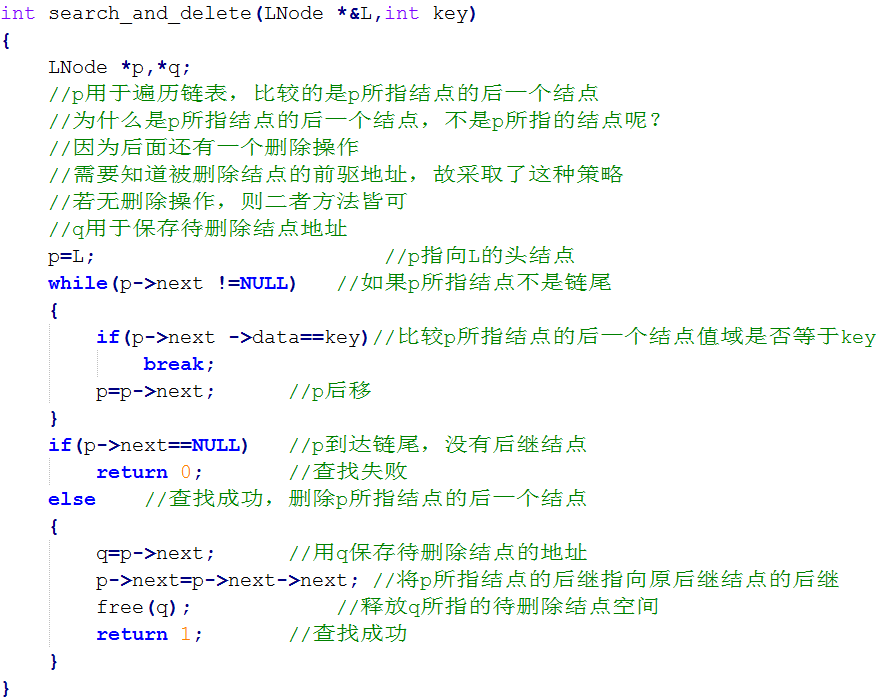
\includegraphics[width=3.22917in,height=2.56250in]{png-jpeg-pics/F334C274192073975B443739BACF94E9.png}
